

%Dati il layout di una metropolitana e la tabella orario dei treni che si vogliono far circolare. Viene definito il modello delle missioni dei singoli treni. Il modello delle missioni unito al modello dello stato della linea formano il modello di scheduling del sistema. 
%Il risultato dell'analisi del model chec ker 

In questo paragrafo descrivero l'approccio utilizzato per verificare e correggere la presenza di deadlock in una metropolitana.
Il nostro approccio si basa sull'utilizzo iterativo di un model checker per verificare la presenza di deadlock di una metropolitana.

\begin{figure}[htp]
	\begin{centering}	
	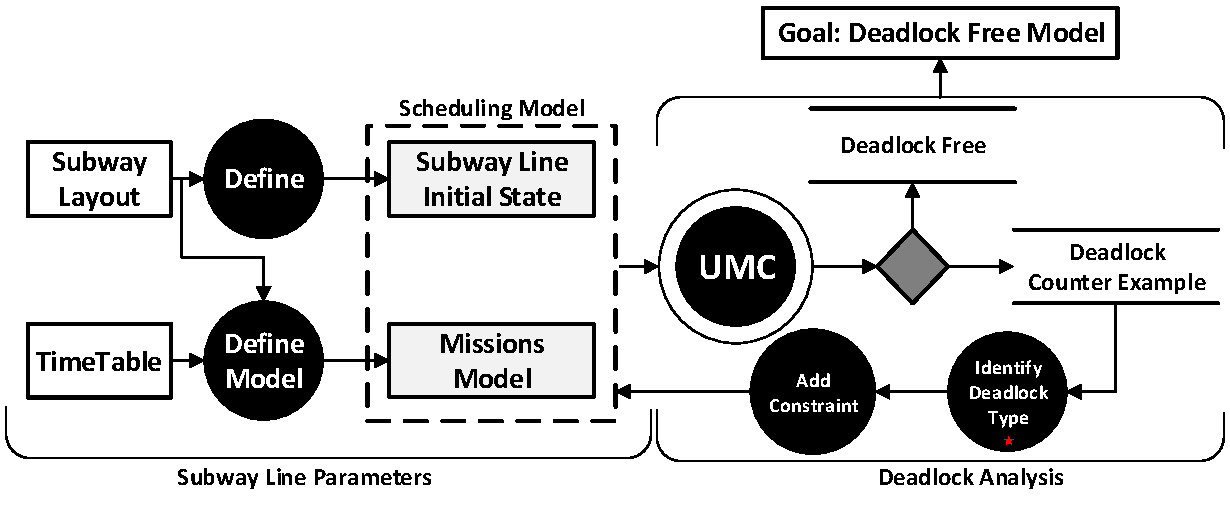
\includegraphics[width=0.45\textwidth, clip]{img/processo}
	\caption{Overview of the approach}
	\label{fig:process}
	\end{centering}
\end{figure}

Nella figura \ref{fig:process} viene descritto graficamente l'approccio usato.

I dati di partenza sono  il layout della metropolitana e la tabella orario dei treni che si vogliono far circolare. Questi dati sono usati per definire
i modelli delle missioni dei singoli treni. 

Il layout della metropolitana viene usato anche per definire lo stato iniziale della linea. Prevedento ad esempio il blocco di alcune aeree perchè impegnate da lavori di manutenzione.